
This chapter gives the general view of our behavioural model-based testing framework for software product lines \cite{Devroey2012} by instantiating the generic process described in Section \ref{sec:mbt}.
The main part of the framework concerns the \emph{abstract test suite selection} at the product line (domain) level. Based on this selection, the test engineer may \emph{prioritize} products to test and/or assess the test suite using \emph{mutation analysis}. We focus on \emph{behavioural} aspect: the selection is done from a \gls{FTS}, defined by the test engineer. 


%%%%%%%%%%%%%%%%%%%%%%%%%
\section{Overview}
%%%%%%%%%%%%%%%%%%%%%%%%%

\begin{figure}[t]
	\centering
	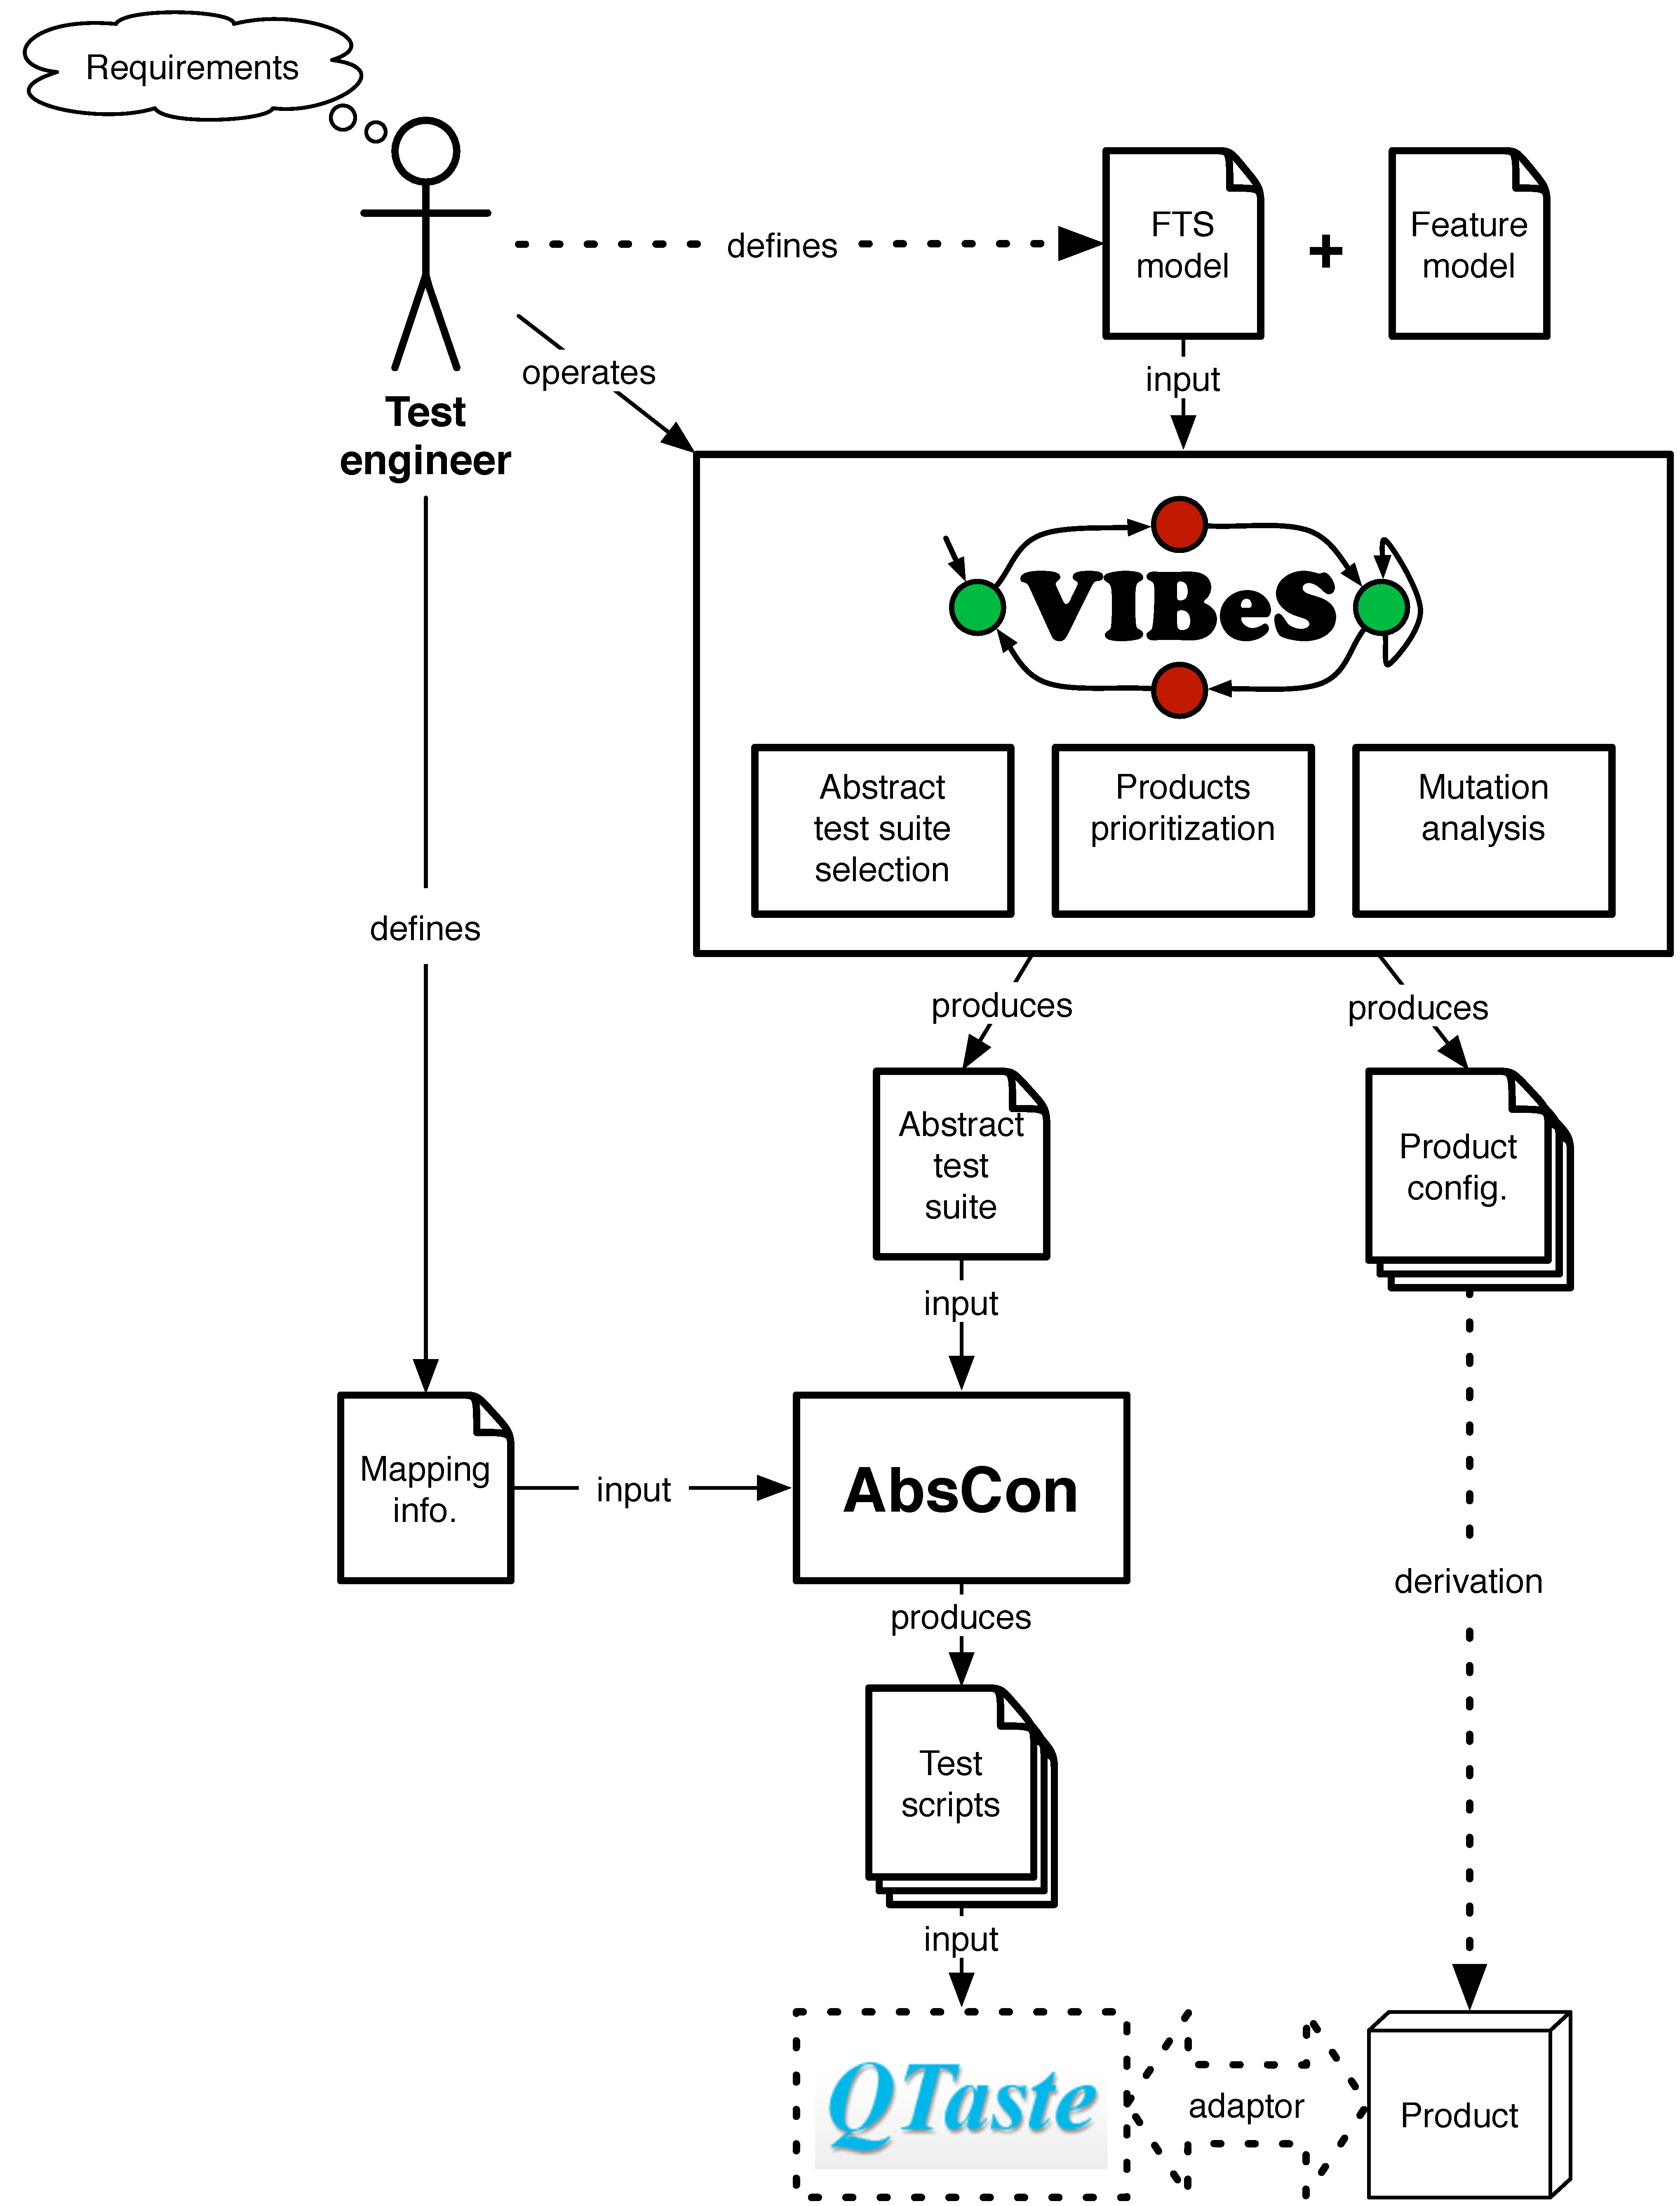
\includegraphics[width=110mm]{framework-overview}
	\caption{Behavioural SPL testing framework overview}
	\label{fig:frameworkoverview}
\end{figure}

\glsreset{VIBeS}

Figure \ref{fig:frameworkoverview} gives a general view of our framework. The test engineer, based on requirements, defines a FTS (and a feature model). This FTS serves as input to our tool: the \gls{VIBeS} framework. The tool is operated by the engineer to select a test suite, based on a selection criterion coming from the requirements. For instance, one may want to select a test suite that covers the states of the FTS or that contains test cases as dissimilar as possible. Based on this test suite, the engineer may prioritize the products to test, \eg by selecting the product that allows to execute as much test cases as possible, and assess the quality of the test suite using mutation analysis. 

\glsreset{AbsCon} \glsreset{QTaste}

Eventually, \gls{VIBeS} produces an \emph{abstract test suite}, with test cases representing sequences of actions from the FTS. This test suite is defined for the product line, which means that the abstract test cases, once concretized, may be executed by one or more products. The \emph{\gls{concretization}} is handled by the \gls{AbsCon} plugin, based on a \emph{mapping} provided by the test engineer. \gls{AbsCon} produces executable test scripts for the \gls{QTaste}, a test case management and execution system that uses an adaptor to handle communication with the product under test. The selection of the test cases to execute on the given product amongst all the test cases of the test suite is done in \gls{QTaste}, based on the list of abstract test cases executable by the selected product.

The different elements of Figure \ref{fig:frameworkoverview} are detailed, discussed, and evaluated in the next chapters: abstract test suite selection and product prioritization are presented in Chapter \ref{chap:coverage}; Chapter \ref{chap:mutation} discuss mutation analysis; Chapter \ref{chap:vibes} presents the implementation and usage of \gls{VIBeS}; and Chapter \ref{chap:concretization} details how concretization may be performed with \gls{AbsCon} to get test scripts executable by \gls{QTaste}. Elements in dashed lines in Figure \ref{fig:frameworkoverview} are out of the scope of this thesis and discussed in the next section.


%%%%%%%%%%%%%%%%%%%%%%%%%
\section{Uncovered aspects}
%%%%%%%%%%%%%%%%%%%%%%%%%

In this thesis, our main goal is to provide a framework to support the testing process. Software product line model-based testing is a complex task that involves many aspects, we identify the followings as out of the scope of this work.

%-------------------------------------
\subsection{Process management}
%-------------------------------------

\gls{VIBeS} is a toolbox that allows to perform various testing activities based on the requirements of the test engineer. In a software engineering context, those activities are organised in process \cite{swebok2014} that has to be managed and monitored. The definition of such product line model-based testing process falls out of the scope of this work.

%-------------------------------------
\subsection{Requirements definition}
%-------------------------------------

We assume that requirements are used both to define the FTS and the feature model, and the test suite selection criterion. The formalism used to define those requirements may take several forms: structured or semi-structured sentences \cite{cucumber}, goal modelling \cite{VanLamsweerde2008}, LTL formulas that the product line must satisfy \cite{Classen2013b}, \etc How those requirements are elicited  and formalised \cite{Bagheri2012,Niu2008,Metzger2014} is out of the scope of this work. We assume that the test engineer knows the requirements  when operating \gls{VIBeS}.

%-------------------------------------
\subsection{FTS model definition}
%-------------------------------------

In its implementation, \gls{VIBeS} allows to define FTSs using a Java DSL or with an XML file. The process used to define this \gls{FTS} model is out of the scope of this work. 

Model the detailed behaviour of the \gls{SPL} using an \gls{FTS} is intractable. Instead, the test engineer abstracts the behaviour to be able to run analysis on the model. This abstraction is done by defining abstract actions (\ie actions that represent one or more effective functions or methods calls) or by focusing on the subset of behaviour under test. As \glspl{FTS} may be used to express the semantic of other variability-aware behavioural languages \cite{Cordy2014}, one may also use an abstract modelling language: \eg FORML \cite{Shaker2012a,Shaker2012}. In such a case, we assume that a bidirectional mapping can be defined between the abstract modelling language and FTS.

%-------------------------------------
\subsection{Feature model definition}
%-------------------------------------

We assume that the feature model used with the \gls{FTS} is a boolean feature model that may be translated to a \gls{CNF} formula \cite{Batory2005,Schobbens2007}. As for \glspl{FTS}, the definition and the formalism used to define this feature model are out of the scope of this work. Considering non-boolean feature models requires to use constraint solvers other than \gls{SAT} or \gls{BDD} solvers, and to adapt \glspl{FTS}' feature expressions to take non-boolean types into account.

%-------------------------------------
\subsection{Product derivation}
%-------------------------------------

\gls{VIBeS} produces a set of product configurations to test. This set is represented as a set of boolean assignments of the feature model. The derivation process of the actual product (in dashed lines in Figure \ref{fig:frameworkoverview}) is out of the scope of this work. This derivation may take several forms and may be automated or not \cite{Pohl2005}.

%-------------------------------------
\subsection{Test scripts execution}
%-------------------------------------

Test scripts management, covering executions of the scripts and reporting, is handled by \gls{QTaste}. \gls{QTaste} is an industrial test environment that provides functionalities to execute test scripts using an adaptor to manipulate the product under test. More details about \gls{QTaste} are provided in Chapter \ref{chap:concretization}.


%%%%%%%%%%%%%%%%%%%%%%%%%%%%%%%%%%%
\section{Wrap up}
%%%%%%%%%%%%%%%%%%%%%%%%%%%%%%%%%%%

This chapter presents an overview as well as the limitations of our behavioural model-based product line testing framework. We assume connected \glspl{FTS} and boolean \glspl{feature model} as inputs. The different elements of the framework are detailed in the next chapters.
